\section{Einleitung}

	Vorverstädnis, Einleitung in die Arbeit

\section{Der Text: Mk 2,\ 1--12}

	\subsection{Übersetzung aus dem Urtext}

		\textit{Auf der Grundlage des Textes des \textsc{Novum Testamentum Graece}\footcite{NA28} wurde der Urtext übersetzt wie folgt:}

			\textsuperscript{Mk 2,\ 1} Und er kam nach einigen Tagen wieder nach Kapernaum und man hörte, daß er in einem Hause sei. \textsuperscript{2} Und es versammelten sich so viele, so daß kein Platz mehr war, auch nicht vor der Tür; und er sagte zu ihnen das Wort. \textsuperscript{3} Und sie kommen und bringen vor ihn einen Gelähmten, der von vieren getragen wurde. \textsuperscript{4} Und weil sie [ihn\footnote{Ergänzung durch d. Vf.}]  wegen der Volksmenge nicht zu ihm bringen können, deckten sie das Dach ab, wo er war, und nachdem sie es aufgegraben hatten, lassen sie das Bett hinunter, darin der Gelähmte lag. \textsuperscript{5} Und weil Jesus ihren Glauben erkannte, sagt er zu dem Gelähmten: \textit{\frqq Kind, deine Sünden werden dir erlassen.\flqq}

			\textsuperscript{6} Es saßen dort aber auch einige der Schriftgelehrten und überlegten in ihren Herzen: \textsuperscript{7} \textit{\frqq Wer ist er, daß er dies sagt? Er lästert. Wer kann Sünden erlassen außer einem, der ist Gott?\flqq} \textsuperscript{8} Und weil Jesus sogleich in seinem Geist erkannte, was sie so bei sich überlegten, sagte er zu ihnen: \textit{\frqq Was überlegt ihr in euren Herzen?} \textsuperscript{9} \textit{Was ist leichter? Dem Gelähmten zu sagen: deine Sünden werden dir erlassen? Oder zu sagen: steh auf, nimm dein Bett und geh umher?} \textsuperscript{10} \textit{Damit ihr aber wißt, daß der Menschensohn Vollmacht hat, auf der Erde die Sünden zu erlassen\flqq} -- sagt er zu dem Gelähmten:

			\textsuperscript{11} \textit{\frqq ich sage dir: steh auf, nimm dein Bett und geh in dein Haus.\flqq} \textsuperscript{12} Und er stand auf und, nachdem er sofort sein Bett genommen hatte, ging er vor allen hinaus, so daß alle staunten und den Gott verherrlichten indem sie sagten: \textit{\frqq etwas derartiges haben wir niemals gesehen.\flqq}

	\subsection{Textkritik}

	\textbf{V. 1} bietet als Varianten {\ibygr{en oikw}} (\textit{Dativ}), welche außerordentlich gut bezeugt ist, vor allem unter den ständigen Zeugen Codex Sinaiticus, der Minuskel 33 und dem Codex Vaticanus, wobei letzterem nicht nur wegen seines Alters (350 n. Chr.) die größte Bedeutung zukommt\footcite[cf.][47]{schnelle2014}. Die zweite Variante {\ibygr{eij oikon}} (\textit{Akkusativ}) wird dagegen hauptsächlich von weniger gewichtigen und auch jüngeren Textzeugen bezeugt.\footnote{5. Jahrhundert: Codex Alexandrinus, um die erste Jahrtausendwende: Minuskeln 28. 565. 579. 700. 1241. 1424. 2542. \textit{l} 2211)} Vermutlich ist diese Textvariante einem Abschreibfehler geschuldet, wobei vermutlich das {\ibygr{-n}} und das {\ibygr{-ij}} sowie das {\ibygr{-w}} und das {\ibygr{-on}} verwechselt wurden; eventuell wurde die Präpsition auch sekundär angepasst. Das Hebräische kennt außerdem keine Kasus und so könnte der Fehler auch in schlichter Unkenntnis des Unterschiedes zwischen Akkusativ und Dativ entstanden sein. Aus den vorgenannten Gründen werden die übrigen Lesarten verworfen.

	In \textbf{V. 2} findet sich eine durch den Codex Alexandrinus zusammen mit dem Codex Rescriptus und diversen Minuskeln belegte Ergänzung {\ibygr{euqewj}}. Dagegen findet sich diese in den Codices Sinaiticus und Vaticanus, beides sehr alte Handschriften von hohem Textwert\footcite[cf.][46f.]{schnelle2014}, sowie die Minuskel 33 nicht. Gemäß dem Grundsatz \textit{lectio brevior potior} wird dieser Zusatz als Ausschmückung des Urtextes verworfen.

	\textbf{V. 3} wird von diversen Handschriften in einer anderen Satzreihenfolge dargestellt, was aber entsprechend der freien Satzstellung der griechischen Sprache grammatikalisch keinen Unterschied macht und vermutlich Abschreibefehlern zugrundeliegt.

	Die Ergänzung {\ibygr{idou andrej}}, bezeugt durch die Minuskel 28, wird nicht nur aufgrund ihres geringen Alters verworfen als \textit{lectio brevior et ergo potior}.

	In \textbf{V. 4} findet sich statt der sehr gut im Codex Vaticanus sowie der Minuskel 33 belegten Lesart {\ibygr{prosenegkai}}, \textit{hervorbringen}, die Variante {\ibygr{proseggisai}}, \textit{sich nähern}, die im Codex Alexandrinus sowie im Codex Rescriptus und außerdem in den Minuskelfamilien \textit{f}\textsuperscript{1.13} sowie diversen weiteren Minuskeln (28, 565, 579, 700, 1241, 1424, 2542) sowie im Lektionar 2211 bezeugt ist. Diese  Variante wird wegen des relativ geringen Textwertes des Codex Alexandrinus in den Evangelien\footcite[cf.][47]{schnelle2014}, des geringen Alters der Minuskeln (datiert in das 9.-13. Jahrhundert) verworfen. Gewichtiger ist aber der Befund, dass die Variante {\ibygr{proseggisai}} vermutlich eine spätere Glättung darstellt, weil {\ibygr{prosenegkai}} kein Objekt trägt, wodurch unklar bleibt, wen die vier Männer bringen wollten; diese Variante wird gegenüber der \textit{lectio difficilior} des Textes verworfen.

	Die Ergänzung {\ibygr{o) Ihsouj}} wird als nur wenig, nämlich durch D, {\ibygr{D}}, {\ibygr{Q}} sowie die Minuskeln 700, 1424 sowie in der Vetus Latina, bezeugte und vermutlich nachträgliche Ergänzung zur Hervorhebung des Subjektes gegenüber der \textit{lectio difficilior et brevior} des Textes, welche folglich überwältigend häufig bezeugt ist, verworfen.

	Neben {\ibygr{o)pou}}, was sehr gut im Codex Sinaiticus, Codex Vaticanus, D, L, Minuskel 892, einzelnen altlateinischen Zeugen sowie in einigen von der Vulgata abweichenden Versionen bezeugt ist, finden sich als Varianten zum einen {\ibygr{ef w)}}, was überschaubar in $\mathfrak{P}$\textsuperscript{84vid}, in den Codices Alexandrinus et Rescriptus belegt ist, sowie {\ibygr{ef ou)}}, was nur wenig, nämlich durch den Codex Coridethianus, die Minuskelfamilie \textit{f}\textsuperscript{13} sowie Minuskeln 33 und 565, belegt ist und schließlich {\ibygr{eij o)n}}, was lediglich im Codex Washingtonianus (4./5. Jahrhundert) belegt ist. Die Variante {\ibygr{o)pou}} sehr gut bereits seit dem 4. Jahrhundert bezeugt; alle anderen Varianten sind nur in deutlich jüngeren Texten belegt oder auch als Abschreibefehler wie z. B. {\ibygr{ou)}} gegenüber {\ibygr{o)n}} und werden daher verworfen.

	In \textbf{V. 5} finden sich als Varianten {\ibygr{idwn de}} und {\ibygr{kai idwn}}, was beides recht umfangreich belegt ist. {\ibygr{idwn de}} wird bezeugt durch den Codex Alexandrinus, D, K, W, {\ibygr{G}}, {\ibygr{D}}, 0130, \textit{f}\textsuperscript{1}, 579, 1242, 1424, 2542, \textit{l} 2211, die Vulgata und einen Teil der altlateinischen Zeugen, die gesamte syrische und einen Teil der sahidischen Überlieferung; {\ibygr{kai idwn}} wird bezeugt durch $\mathfrak{P}$\textsuperscript{88}, die Codices Sinaiticus, Vaticanus et Rescriptus, L, Coridethianus, die Minuskelfamilie \textit{f}\textsuperscript{13}, die Minuskeln 33, 565, 700, 892, den anderen beiden Synoptikern, in einigen Handschriften der sahidischen Überlieferung sowie in der bohairischen Überlieferung. Der Vorzug wurde vorliegend aber der Variante {\ibygr{kai idwn}} gegeben, da diese einerseits auf einem älteren Textbestand beruht und andererseits auch wortgleich bei den anderen beiden Synoptikern zu finden ist\footnote{cf. Mt 9, 4 et Lk 5, 20.}.

	Weiter finden sich die Varianten {\ibygr{afewntai}}, {\ibygr{afiwntai}}, {\ibygr{afiontai}}, {\ibygr{afientai}}. Nachdem die Variante {\ibygr{afientai}} jedoch gegenüber den anderen außerordentlich gut durch den Codex Vaticanus, die Minuskeln 0130, 28, 33, 565, 1241 und das Lektionar 2211 sowie beinahe allen lateinischen Traditionen bezeugt ist und die Variante {\ibygr{afewntai}} dem ionischen Dialekt entstammt, aber bedeutungsunerheblich ist, werden die verbliebenen beiden Varianten als Abschreibefehler, vielleicht aus Unkenntnis des Kopisten der griechischen Sprache überhaupt, verworfen.

	In \textbf{V. 7} werden die Varianten {\ibygr{o)ti}} und {\ibygr{ti}} geboten. Wohingegen die letztere überwältigend häufig bezeugt ist weichen lediglich der Codex Vaticanus sowie der Codex Coridethianus davon ab und lesen {\ibygr{o)ti}}. Obschon dem Codex Vaticanus eine hohe Textqualität zugesprochen wird\footcite[cf.][XVII]{elbtk2017} ergibt sich aus seiner Verwandschaft zum Beispiel mit $\mathfrak{P}$\textsuperscript{75}\footcite[cf.][XVII]{elbtk2017} aus dem 3. Jahrhundert, welches diese Lesart gerade nicht bezeugt und welchem ebenfalls ein hohes Maß an Textqualität zugesprochen wird\footcite[cf.][46]{schnelle2014}, dass die Lesart {\ibygr{ti}} wahrscheinlich die ursprünglichere ist.

	Außerdem steht bei den anderen beiden Synoptikern am Ende des Fragesatzes {\ibygr{blasfhmiaj}}, was aber als \textit{Lectio longior et ergo peior} bzw. als Ausschmückung verworfen wird.

	In \textbf{V. 8} ist das im Text stehende {\ibygr{ou(twj}} im Codex Vaticanus sowie W, {\ibygr{Q}}, in der Peschitta sowie in einzelnen sahidischen Handschriften ausgelassen. Obschon der Codex Vaticanus ein Text von hoher Qualität ist, sind die übrigen Bezeugungen später datiert. Es ist denkbar, dass diese Auslassung ein Homoioarkton ist, also wegen dem gleichen Beginn von {\ibygr{autou}}, {\ibygr{ou(twj}}, {\ibygr{e(autoij}} und {\ibygr{autoij}}. Daher wird diese Variante der Auslassung verworfen.

	Die Einfügung {\ibygr{autoi}}, die vielfältig von $\mathfrak{P}$\textsuperscript{84vid}, den Codices Alexandrinus, Rescriptus, K, {\ibygr{G}}, der Minuskelfamilie \textit{f}\textsuperscript{13}, den Minuskeln 33, 1242, 1424, dem Lektionar \textit{l} 2211, dem Mehrheitstext sowie der Harklensis bezeugt ist, wird als \textit{Lectio longior et ergo peior} verworfen.

	Die Auslassung von {\ibygr{autoij}} ist lediglich im Codex Vaticanus, in {\ibygr{Q}} sowie ff\textsuperscript{2} bezeugt. Diese Variante wird wegen der schieren Überzahl der positiven Bezeugungen aus ähnlichen Gründen wie oben bei {\ibygr{ou(twj}} als Homoioarkton verworfen.

	In \textbf{V. 9} steht anstelle von {\ibygr{afientai}} in einigen Handschriften {\ibygr{afewntai}}. Diese Variante wird aus denselben Gründen der textkritischen Entscheidung oben in Vers 5 als Abschreibe- bzw. als Hörfehler verworfen.

	Statt {\ibygr{egeire}} findet sich überschaubar bezeugt {\ibygr{egeirou}}. Dies könnte ebenfalls als Abschreibe- bzw. Hörfehler sein. Jedoch ist {\ibygr{egeirou}} auch zugleich der attische Imperativ, was aber, wie oben bei Vers 6 dargelegt, hier ebenfalls bedeutungsunerheblich ist und zugleich auch der Sprachunkenntnis des Kopisten geschuldet sein kann. Die Variante wird daher verworfen.

	{\ibygr{kai aron ton krabatton sou}} wird bisweilen in einer anderen Reihenfolge bezeugt, was aber ohne Bedeutung ist. Teilweise fällt das {\ibygr{kai}} vermutlich in Angleichung an Mt 9,6 fort\footcite[cf.][51]{schnelle2014}, unter anderem bezeugt durch die Minuskel 33, aber auch den Codex Rescritpus oder den Codex Bezae Cantabrigiensis. In der Minuskel 700 fällt gar {\ibygr{aron}} fort, dies aber vermutlich als Homoioteleuton.

	Statt {\ibygr{peripatei}}, \textit{geh umher}, findet sich {\ibygr{u)page}}, \textit{geh weg}, bezeugt durch $\mathfrak{P}$\textsuperscript{88}, Codex Sinaiticus und Weitere, was sich ebenfalls in Mt 9,6 findet, weshalb vorliegend erneut eine sekundäre Angleichung an Mt angenommen, diese Lesart mithin verworfen wird\footcite[cf.][51]{schnelle2014}.

	\textbf{V. 10} {\ibygr{afienai a)martias epi thj ghj}} wird teilweise in anderer Reihenfolge bezeugt. Durch die Umstellung von {\ibygr{afienai a)martias} an den Schluss des Satzteiles wird {\ibygr{epi thj ghj}}, also die universelle Vollmacht Jesu, betont: \textit{..., dass der Menschensohn \textbf{auf der Erde} Vollmacht hat, die Sünden zu erlassen.} So bezeugen  $\mathfrak{P}$\textsuperscript{88}, Codex Sinaiticus, Codex Rescriptus, Codex Bezae Cantabrigiensis, einige Minuskelhandschriften, darunter \textit{33}, die lateinische Vulgata, die syrische Peschitta und weitere Übersetzungen. Die Stellung {\ibygr{afienai epi thj ghj a)martias}} betont gleichfalls Jesu universelle Vollmacht (dies wird bei der Interpretation noch eine Rolle spielen). Sie bezeugen der Codex Alexandrinus sowie \textit{f}\textsuperscript{1,13}. In wenigen Handschriften -- nämlich W, b und q -- wird {\ibygr{epi thj ghj}} gar ganz ausgelassen, was aber vermutlich ein Homoioteleuton mit {\ibygr{legei}} darstellt. Vorliegend wird aber der im Text nachgewiesenen Reihung der Vorzug gegeben, da der diese Textfassung belegende Codex Vaticanus der wesentlich ältere Text gegenüber den anderen Varianten ist\footcite[cf.][47]{schnelle2014}. Daher werden die Varianten verworfen.

	In \textbf{V. 12} wird anstelle von {\ibygr{emprosqen}} sinnähnlich durch die Codices Alexandrinus, Rescriptus et Bezae Cantabrigiensis, die Minuskelfamilien \textit{f}\textsuperscript{1.13} und das Lektionar 2211 {\ibygr{enantion}} bezeugt sowie {\ibygr{enwpion}} durch den Codex Coridethianus aber auch u.a. die Minuskeln 28, 33.
	{\ibygr{enwpion}} könnte ein Hör- bzw. Abschreibefehler von {\ibygr{enantion}} sein. Dies wird auch dadurch gestützt, dass die Überlieferungen von {\ibygr{enwpion}} allesamt um das 9. Jahrhundert datiert werden, diejenigen von {\ibygr{enantion}} sind jedoch deutlich älter, nämlich durch die Codices Alexandrinus Rescriptus et Bezae Cantabrigiensis auf das 4. Jahrhundert datiert.
	{\ibygr{enantion}} ist gegenüber {\ibygr{emprosqen}}, so u.a. belegt durch die Codixes Sinaiticus et Vaticanus sowie die Minuskeln 579, 700 und 892, deutlich schwächer belegt, da der Codex Vaticanus die älteste Pergamenthandschrift ist, die anderen Textzeugen sind neueren Datums. Von der inneren Textkritik her ist die Variante {\ibygr{emprosqen}} wahrscheinlicher, bedeutet es doch \textit{vor} -- wohingegen {\ibygr{enantion}} \textit{gegenüber} (mit einer Nuance der Feindlichkeit oder Gegnerschaft) meint.
	Daher werden beide Varianten verworfen.

	{\ibygr{legontaj}} wird in wenigen Handschriften ausgelassen, in der überwiegenden Mehrheit und quer durch alle Handschriftgattungen jedoch ist es belegt. Daher wird die Variante der Auslassung verworfen.

	Die teilweise überlieferte Umstellung von {\ibygr{ou)twj oudepote}} nach {\ibygr{oudepote ou)twj}} wird als Abschreibefehler verworfen.

\section{Textanalyse und Literarkritik}

	\subsection{Einleitungsfragen}

		Das Markusevangelium entstand \glqq entweder \textit{kurz vor oder kurz nach 70 n. Chr.}\grqq, da sich Mk 13,\ 2.14 sowohl als Bezug auf die Zerstörung des jerusalemer Tempels durch die Römer als auch als entsprechende Prophezeiung verstehen läßt\footcite[269]{schnelle2013}.

		Sein Verfasser, der aufgrund der semitischen Färbung seiner Sprache vermutlich zweisprachig griechisch-aramäisch gewesen war\footcite[cf.][275]{dschulnigg1986}, war wohl eher ein ansonsten unbekannter Christ mit dem Namen Markus\footcite[cf.][267]{schnelle2013} als der Dolmetscher des Petrus, wie von Papias von Hierapolis berichtet\footcite[cf.][266]{schnelle2013}. Die genaue Verfasserschaft bleibt aber letztlich unklar.

		Der Abfassungsort lässt sich aufgrund vieler Latinismen\footcite[cf.][268]{schnelle2013}\footcite[cf.][277ff.]{dschulnigg1986} (z.B. Mk 12, 14 \textit{cenus}, \textit{flagellare}) im Evangeliumstext auf Rom eingrenzen, wobei die Latinismen ebenfalls aufgrund der herrschenden römischen Weltmacht ihren Einzug in Mk gefunden haben könnten\footcite[cf.][268]{schnelle2013}.

		Obschon der Abfassungsort Rom als gesichert gelten kann, sind gleichwohl die Adressate vermutlich nicht Mitglieder der römischen Gemeinde gewesen. Der Adressatenkreis war wohl eher eine heidenchristliche Gemeinde\footcite[cf.][270]{schnelle2013}. Hinweise hierfür sind die Erklärung jüdischer Bräuche, z. B. Mk 7, 3f. (Händewaschung) und Mk 14, 12 (Schlachten des Passalammes), und Begriffe, z. B. Mk 5, 41 (\RL{_tlyt' qwmy}), Mk 7, 34 ({\ibygr{effaqa}}) und Mk 15, 34 (\RL{'ly 'ly lmh `zb.tny}).

	\subsection{Abgrenzung der Perikope}

		Nunmehr soll die Frage der Abgrenzung der Perikope im Markus-Evangelium behandelt werden.

		Nach hinten ist die Perikope abgegrenzt durch den erneuten Einsatz mit dem Bericht von Jesu Reise nach Kapernaum, es findet also ein Orts- und Zeitwechsel (\textit{\glqq nach einigen Tagen\grqq}) statt.

		Nach vorne ist die Perikope gleichfalls abgegrenzt durch einen Ortswechsel in V. 13: \textit{\glqq Und er ging wieder hinaus nahe des Sees [...]\grqq}.

	\subsection{Kontextanalyse}

		Das Markusevangelium ist das zweite der vier Evangelien und steht am Beginn des Neuen Testamentes. Die Evangelien widmen sich in je eigener Weise dem Leben, Wirken und Sterben Jesu Christi. Wie noch zu erörtern ist, ist das Markusevangelium nach der \textit{Zwei-Quellen-Hypothese} vermutlich neben der \textit{Logienquelle} die literarische Grundlage des Matthäus- und Lukasevangeliums. Aufgrund dieser wahrscheinlichen literarischen Abhängigkeit untereinander werden diese auch \textit{Synoptische Evangelien} genannt. Das Johannesevangelium ist in Inhalt und Aufbau davon gesondert zu betrachten.

		Das Markusevangelium wird nach \cite{bormann2014}\footcite[224]{bormann2014} gegliedert wie folgt:

		\paragraph{1--8,26 Jesu Wirken in Galiläa}

			\begin{itemize}
				\item \textbf{1,1--15.} Der Täufer und Jesus
				\item \textbf{1,16--3,6.} Jünger, erste Heilungen, erste Konflikte
				\item \textbf{3,7--6,56.} Jesu große Taten und Reden
				\item \textbf{7,1--8,26.} Hinwendung zu den Heiden
			\end{itemize}

		\paragraph{8,27--10 Jesu Weg nach Jerusalem}

			\begin{itemize}
				\item \textbf{8,27--9,13.} Die Person Jesu
				\item \textbf{9,14--10.} Das Leben in der gemeinde
			\end{itemize}

		\paragraph{11--16 Jesu Wirken in Jerusalem}

			\begin{itemize}
				\item \textbf{11,1--25.} Jesu Auftreten in Jerusalem und im Tempel
				\item \textbf{11,27--12,44.} Jesus lehrt im Tempel
				\item \textbf{13.} Die apokalyptische Rede
				\item \textbf{14,1--14,42.} Jesus und die Jünger
				\item \textbf{14,43--15,41.} Gefangennahme, Prozeß und Hinrichtung Jesu
				\item \textbf{15,42--16.} Das Grab
			\end{itemize}

	\subsection{Gliederung der Perikope}

		Die Perikope wird in drei Abschnitte bzw. narrativ in Szenen gegliedert:

		\paragraph{I.} Vv. 1--5: Jesu Auftritt in Kapernaum, Predigt, Vorstellung des Gelähmten und Ansprache durch Jesus.

		\begin{enumerate}
			\item (V. 1) Jesus kommt nach Kapernaum.
			\item (V. 2) Es versammelten sich viele, Jesus predigt ihnen.
			\item (Vv. 3f.) Sie bringen ihm den Gelähmten und decken dafür das Dach ab.
			\item (V. 5) Jesus spricht den Gelähmten an und vergibt ihm seine Sünden
		\end{enumerate}

		\paragraph{II.} Vv. 6--10: Streitgespräch mit den Pharisäern.

			\begin{enumerate}
				\item (V. 6) Einführung der Schriftgelehrten
				\item (V. 7) Fragen der Schriftgelehrten in ihren Gedanken
				\item (V. 8ff.) Entgegnung Jesu
			\end{enumerate}

		\paragraph{III.} Vv. 11--12: Erneute Ansprache Jesu, Aufstehen des Gelähmten, Staunen des Volkes.

		\begin{enumerate}
			\item (Vv. 11, 12a.) Jesus fordert den Gelähmten zum Aufstehen und Gehen auf; er steht auf und geht.
			\item (V. 12b) Das Volk staunt.
		\end{enumerate}

	\subsection{Textpragmatik}

	Jeder Text hat eine bestimmte Funktion, daher stellt sich immer auch die Frage nach der Textpragmatik, also des {\ibygr{pragmatoj}}, des Dings, der Sache, des Geschehens eines Textes, vorliegend geht es um Anlaß, Ziel und Wirkung des Textes.

	Der Evangelist Markus beginnt bereits in V. 1: \glqq Dies ist der Anfang des Evangeliums von Jesus Christus, dem Sohn Gottes.\grqq Der Begriff {\ibygr{euaggelion}}, \textit{frohe Botschaft} findet sich, wenn auch selten, bereits in der Septuaginta und zwar dann, wenn einem König ein militärischer Sieg übermittelt wurde, etwa 2Sam 18, 20--27. Das Verb {\ibygr{euaggelizein}}, \textit{eine Frohbotschaft verkünden} jedoch kommt häufiger vor, vor allem bei Jesaja und in 2Sam 4, 10. Auch sonst ist Evangelium als Fachausdruck in der Antike bekannt\footcite[cf.][2]{dormeyer2008}.

	Der Begriff des Evangeliums als \glqq frohe (Sieges)botschaft\grqq scheint freilich dem Inhalt des Markusevangelium zunächst entgegenzustehen.

	So ist die Jesusüberlieferung in Mk auf die Passion hin zugespitzt\footcite[cf.][107]{niebuhr2011}, in der ja das scheinbare Scheitern Jesu zum dargestellt ist. Auf dem Weg dorthin erlebt Jesus diverse Konflikte mit der jüdischen Obrigkeit, stellt sich aber zugleich als \glqq der Jesus der vollmächtigen \glq Lehre\grq\grqq\footcite[107]{niebuhr2011} dar, als den Sohn Gottes, als den Menschensohn.
	Dieser starke, vollmächtige und göttliche Jesus \textit{Christus} ist es aber auch, der \glqq in der Passion scheinbar scheitert\grqq\footcite[cf.][108]{niebuhr2011}.
	Doch das ist gerade die Absicht des Evangelisten Markus: Jesus als vollmächtigen Gott darzustellen, der aber zugleich auch (leidender, sterbender) Mensch ist. Dazu wird noch mehr zu sagen sein.

	Die vorliegende Perikope fügt sich hinsichtlich ihrer Pragmatik nahtlos in das Mk-Gesamtprogramm ein. Zum göttlichen Jesus wird ein Gelähmter gebracht, ihm werden die Sünden vergeben und er wird geheilt. Das, wie noch zu zeigen ist, nachträglich eingefügte Streitgespräch zieht die Geschichte gewissermaßen zurück auf \textit{menschlichen} \glqq Boden der Tatsachen\grqq (wogegen sich Jesus ja dann unter Bezug auf seine {\ibygr{exousian}} dann wiederum wehrt.)

	Diese hier und anderswo erkennbare \glqq Verschränkung von Niedrigkeit und Hoheit Jesu\grqq\footcite[108]{niebuhr2011} darzustellen ist Ziel und Anlaß des Markusevangeliums.

	\subsection{Quellenkritik, Synoptischer Vergleich}

	Alte Texte, wie vorliegend eines Evangeliums, müssen immer auch hinsichtlich ihrer Quellen befragt werden, was im Folgenden geschehen soll.

	In der Evangelienexegese ist ein Umstand besonders auffällig: Die Evangelien Matthäus, Markus und Lukas sind in hohem Maße literarisch von einander abhängig und stimmen in weiten Teilen inhaltlich und strukturell überein\footcite[cf.][83]{niebuhr2011} -- daher man sie auch \textit{synoptische Evangelien} nennt --, wohingegen alle drei auch ihnen exklusiven Textbestand besitzen (sog. Sondergut) bzw. gegenüber den anderen Inhalte auslassen (sog. Lücken). Um das Verhältnis dieser drei synoptischen Evangelien untereinander besser beschreiben zu können, wurde die \textit{Zwei-Quellen-Theorie} entwickelt. Diese fußt zum einen wegen seines Alters auf der Priorität des Markus und zum anderen auch auf der so genannten Logienquelle.

	Bemerkenswert ist, daß \glqq die drei Evangelien sowohl im Wortbestand wie in der Anordnung einander am nächsten sind, wo sie mit dem [...] Markusevangelium parallel gehen\grqq\footcite[84]{niebuhr2011}; deshalb, und weil es als das älteste Evangelium angesehen wird\footcite[cf.][210]{schnelle2013}, wird Mk als die \textit{erste} und wichtigste \textit{Quelle} der beiden betrachtet (\glqq Markuspriorität\grqq\footcite[84]{niebuhr2011}\footcite[ibid.]{schnelle2013}). Es wird angenommen, daß Mt und Lk wesentliche Inhalte von Mk übernommen und diesen womöglich verbessert haben\footcite[cf.][213]{schnelle2013}.

	Bei dem verbleibenden Textbestand von Mt oder Lk, der also nicht Inhalt von Mk ist, gibt es eine zweite Schnittmenge, die sog. \textit{Logien-Quelle} (\textit{Q}), und welche die zweite Quelle darstellt. Es wird angenommen, daß es sich hierbei um wörtliche Aussprüche Jesu handelt.

	Es gibt ferner auch noch matthäisches bzw. lukanisches Sondergut, also Texte, die sich weder in Mk noch in Q finden\footcite[cf.][216]{schnelle2013}, wobei man bei deren Einbeziehung dann eigentlich zu einer Vier-Quellen-Theorie gelänge.

	Die Zwei-Quellen-Theorie (eigentlich Vier-Quellen-Theorie) läßt sich also grafisch folgendermaßen darstellen\footcite[Grafik und Beschriftung entnommen aus][84]{niebuhr2011}:

	\begin{center}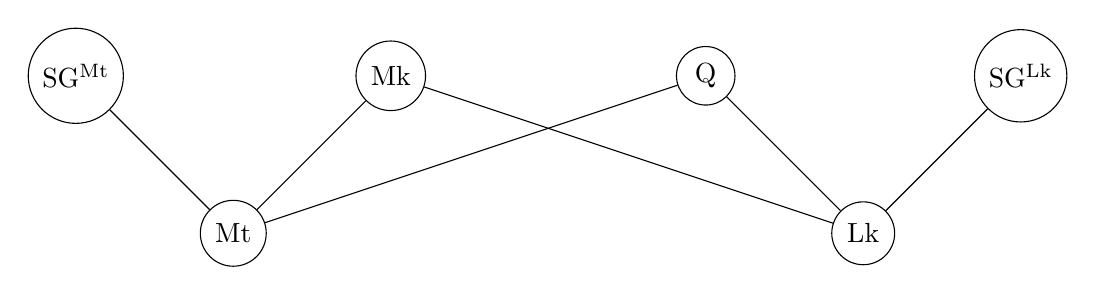
\begin{tikzpicture}[scale=2]
		% Knoten
		\node (Mk) at (3,1) [circle,draw] {Mk};
		\node (Q) at (5,1) [circle,draw] {Q};
		\node (Mt) at (2,0) [circle,draw] {Mt};
		\node (Lk) at (6,0) [circle,draw] {Lk};
		\node (SGLk) at (7,1) [circle,draw] {SG\textsuperscript{Lk}};
		\node (SGMt) at (1,1) [circle,draw] {SG\textsuperscript{Mt}};

		% Kanten
		\draw[-] (SGMt) to (Mt);
		\draw[-] (Mk) to (Mt);
		\draw[-] (Mk) to (Lk);
		\draw[-] (Q) to (Mt);
		\draw[-] (Q) to (Lk);
		\draw[-] (SGLk) to (Lk);
	\end{tikzpicture}\end{center}

	Ein Problem der Zwei-Quellen-Theorie ist aber, daß es durchaus auch markinisches Sondergut gibt. Dieses läßt sich nicht immer mit einer redaktionellen Tätigkeit von Mt oder Lk erklären. So lassen sich einige Auslassungen aus Gründen einer möglichen Anstößigkeit erklären, so etwa Mk 7 (Heilung eines Tauben) oder auch Mk 3 (Meinung der Verwandten, Jesus sei wahnsinnig). Das Fehlen des Gleichnisses von der selbstwachsenden Saat (Mk 4) bei Mt und Lk läßt sich so aber nicht begründen\footcite[cf.][213]{schnelle2013}.

	Ein weiteres Problem der Zwei-Quellen-Theorie sind die sog. \textit{\glqq minor agreements\grqq} zwischen Mt und Lk gegen Mk, was auch ein Hauptgegenargument gegen die Zwei-Quellen-Theorie überhaupt ist\footcite[cf.][84]{niebuhr2011}. Diese so genannten \textit{minor agreements} sind zum teil sprachliche

	Ein anderes Problem ist auch die so genannte \textit{lukanische Lücke}, also daß Lk den Stoff aus Mk 6,45--8,26 (der Seewandel bis zur Heilung des Blinden) vollständig ausgelassen hat. Hätte Lk das Markusevangelium in der heutigen Fassung vorgelegen, wäre dies kaum zu erklären\footcite[cf.][213]{schnelle2013}.

	Ein letztes Problem ist auch, daß Jesus nicht griechisch sprach sondern aramäisch. Eine griechische Logiensammlung mag es also gegeben haben, sie war dann aber nicht unbedingt ursprünglich. Man müßte deshalb vor allem eine aramäische Logienquelle annehmen bzw. suchen. Denkbar ist aber auch, daß die angenommene Logienquelle in sich nicht einheitlich ist\footcite[][]{schnelle2013}.

	Es gab und gibt verschiedene Versuche, diese Probleme zu lösen, etwa durch Annahme, das heutige, kanonische Mk wurde hin zu einem eigeständigen oder als redaktionelle Version existierenden \glqq Deuteromarkus\grqq\ überarbeitet\footcite[cf.][215f.]{schnelle2013} und um sein Sondergut gekürzt, wobei DtoMk wiederum die Grundlage für Mt und Lk gewesen sein könnte.

	Zusammenfassend läßt sich also sagen, daß die Zwei-Quellen-Theorie aufgrund der Vielzahl ihrer Probleme und der dadurch erzwungenen Annahmen nicht stärker oder überzeugender wird. Dennoch ist sie der aktuelle Quasi-Standard in der exegetischen Wissenschaft. Wenn sie schon nicht alle Fragen beantwortet und aufgrund der vielfältigen Annahmen eben nicht besonders belastbar ist, so ist sie doch hilfreich, die Beziehungen der Synoptiker untereinander wenigstens ansatzweise zu verstehen.

	Deshalb wollen wir die vorliegende Perikope mit ihren Parallelstellen bei den beiden anderen Synoptikern vergleichen und wenden hierfür die Zwei-Quellen-Theorie an. Die Gliederung in Szenen hiernach basiert auf der narrativen Analyse unter 3.4. Angaben zum Wortlaut beziehen sich auf den Urtext.

		\subsubsection*{Szene 1. Jesus kommt nach Kapernaum; Mk 2, 1}

		Lk 5, 17 erwähnt keine Ortsangabe, als ob die Perikope mitten am Weg stattfände, erwähnt aber bereits hier gegen Mk die Anwesenheit der Schriftgelehrten und ergänzt die Pharisäer.
		Mt 9, 1 lässt Jesus in ein Boot steigen und fahren in {\ibygr{thn idian polin}}, \textit{seine eigene Stadt}.

		\subsubsection*{Szene 2. Versammlung des Volkes, Jesu Predigt; Mk 2, 2}

		Mt läßt diese Szene ganz aus.
		Lk 5, 17 äußert sich nicht zu einer Versammlung (erst später in V. 19), ergänzt aber das Ausgehen der Kraft des Herrn von Jesus, die jedermann hilft.

		\subsubsection*{Szene 3. Herbeibringen des Gelähmten, Abdecken des Daches; Mk 2, 3f.}

		Mk 2, 3f. wechselt ins Präsens.
		Mt 9, 2 erzählt die Geschichte auf die wesentlichen Aspekte reduziert und hat die Anzahl der den Gelähmten tragenden Männer nicht übernommen. Mk 2, 4 wird von Mt nicht übernommen. Statt des markinischen {\ibygr{krabbatoj}}, \textit{Matte}, schreibt Mt wie auch Lk etwas vornehmer {\ibygr{klinh}}, \textit{Bett}.
		Auch Lk 5, 18f. spricht davon, daß der Gelähmte von \glqq etlichen Männern\grqq\ gebracht wurde -- und nicht von vieren wie Mk. Diese versuchten, den Gelähmten vor Jesus hinzulegen. Daß dafür das Dach abgedeckt werden mußte, Mk 2, 4, erwähnt er nicht.

		\subsubsection*{Szene 4. Jesu Ansprache an den Gelähmten, Sündenvergebung; Mk 2, 5}

		Mk 2, 5a wird von Lk 5, 20a und Mt 9, 2b weitgehend übereinstimmend überliefert.

		In Mk 2, 5b und Mt 9, 2c spricht Jesus den Gelähmten an mit {\ibygr{teknon}}, \textit{Kind}.
		In Lk 5, 20b hingegen spricht er {\ibygr{anqrope}}, \textit{Mensch}.
		Mt ergänzt {\ibygr{qarsei}}, \textit{sei getrost} oder \textit{hab Vertrauen}.

		\subsubsection*{Szene 5. Einführung der Schriftgelehrten, deren Kritik, Antwort Jesu; Mk 2, 6}

		Bei Mk 2, 6 und Mt 9, 3a sind nur wenige (\glqq etliche\grqq) Schrifgelehrte anwesend, wohingegen Lk 5, 21a die Anwesenheit aller Schriftgelehrter impliziert wird. Bei Mk und Mt sprechen die Schriftgelehrten bei sich selbst, sie denken also nur. Bei Lk klingt es hingegen so, als hätten alle Schriftgelehrten (laut) diskutiert.

		\subsubsection*{Szene 6. Einführung der Schriftgelehrten, deren Kritik, Antwort Jesu; Mk 2, 7}

		Die Frage in Mk 2, 7 erscheint bei Mt 9, 3b nicht, bei Lk 5, 21b nutzt den selben Wortlaut wie Mk.

		\subsubsection*{Szene 7. Einführung der Schriftgelehrten, deren Kritik, Antwort Jesu; Mk 2, 8ff.}

		In Mk 2, 8 \glqq erkennt\grqq\ Jesus die Gedanken der Schriftgelehrten, wohingegen er sie bei Mt 9, 4 \glqq sieht\glqq\ und bei Lk 5, 22 \glqq bemerkt\grqq.

		Mk 2, 9, Lk 5, 23 und Mt 9, 5 haben etwa denselben Wortlaut. wobei Mk den die Sündenvergebung noch konkreter mit der Situation verbindet, indem er neben der Aufforderung aufzustehen auch die Aufforderung des Mitnehmens des Bettes anführt.

		Mk 2, 10 stimmt im Wortlaut mit Lk 5, 24a und Mt 9, 6a überein. Mt ergänzt lediglich {\ibygr{tote}}, Lk spricht, wie auch sonst, statt vom {\ibygr{paralutikoj}} vom {\ibygr{paralelumenoj}}, beides \textit{Gelähmter}.

		\subsubsection*{Szene 8. Aufforderung an den Gelähmten und dessen Aufstehen; Mk 2, 11.12a}

		Mk 2, 11.12a, Lk 5, 24b.25, Mt 9, 6b stimmen von der Bedeutung her weitestgehend und abgesehen vom Vokabular überein. Bei Lk preist der Gelähmte Gott, bei Mt nimmt er sein Bett nicht mit.

		\subsubsection*{Szene 9. Das staunende Volk; Mk 2, 12b}

		Mk 2, 12b, Lk 5, 26 und Mt 9, 8 sind ebenfalls weitestgehend deckungsgleich. Bei Mt preist das Volk jedoch Gott, weil er solche Macht \textit{den Menschen} ({\ibygr{toij anqropoij}}, Dativ Plural) gegeben hat, wohingegen Mk und Lk die Verwunderung des Volkes über diese Handlung hervorstellen.

		\subsubsection*{Auswertung der Befunde}

		Vorliegend scheint es gewiß zu sein, dass Mt und Lk als Vorlage den Mk-Text verwendet haben. Daß Teile der außermarkinischen Überlieferung der Quelle Q entstammen können, ist unwahrscheinlich, Mt und Lk nicht gegen Mk übereinsteimmen, mithin keine \textit{major agreements}\footcite[157]{ebner2007}

	\subsection{Literarkritik}

		\subsubsection{Beobachtungen}

		In literarkritischer Hinsicht ist festzustellen:

		Erstens die Doppelung von {\ibygr{legei tw paralutikw}} in den Vv. 5.10, wobei damit in V. 10 nach dem Streitgespräch mit den Schriftgelehrten die erneute Anrede an den Gelähmten eingeleitet wird.

		Außerdem die doppelte Verwendung von {\ibygr{afientai sou a(i a(martiai}} in den Vv. 5.9, wobei sie beim ersten Auftreten von Jesus direkt an den Gelähmten gerichtet werden, beim zweiten Auftreten jedoch gegenüber den Schriftgelehrten im Streitgespräch erwähnt. Diese Doppelung geschieht in V. 9 vermutlich, um das Streitgespräch mit der Heilungserzählung zu verklammern.

		Schließlich die Wiederholung {\ibygr{egeire}} ({\ibygr{kai}}) {\ibygr{aron ton krabbaton sou kai peripatei}} bzw. {\ibygr{u(page eis ton oikon sou}} in Vv. 9.11. In V. 9 wiederum werden diese Worte im Streitgespräch gebraucht, in V. 11 gegenüber dem Gelähmten geäußert\footcite[cf.][172]{ebner2007}. Diese Wiederholung geschieht aus denselben Gründen wie die oben genannte.

		Widersprüchlich ist die Angabe vin V. 12, daß {\ibygr{existastqai}} \textbf{{\ibygr{pantaj}}} {\ibygr{kai doxazein ton qeon}}, \textit{\textbf{alle} staunten und Gott verherrlichten}. Dabei ist doch gerade in Vv. 6--10 eine Gruppe Schriftgelehrter anwesend, die darüber ja eben gerade nicht staunten und Gott deshalb verherrlichten. Dieser Widerspruch hat ja auch Lk zu seiner Ergänzung in Lk 5, 17 veranlaßt und die Schritgelehrten gleich mit in der Einleitung der Perikope genannt\footcite[cf.][172]{ebner2007}. Dies spricht für eine Nachträgliche Einfügung von Vv. 6--10.

		Brüchig ist auch der wechselseitige Bezug der Verse zueinander. Die Vv. 1--5.11f. benötigen für ihre Integrität die Vv. 6--10 nicht, umgekehrt ist diese aber sehr wohl der Fall\footcite[cf.][173]{ebner2007}. Auch dies spricht für eine nachträgliche Einfügung der Vv. 6--10.

		Weiterhin findet sich ein Bruch zwischen Vv. 2.3 durch den Subjektwechsel von {\ibygr{polloi}} zu den vieren, die den Gelähmten tragen. Dies weist auf eine weitere Schicht in V. 3 hin.

		Es findet sich daneben ein Bruch zwischen V. 3, da vier Menschen den Gelähmten bringen, ihn aber in V. 4 eben nicht bringen können und deshalb das Dach abdecken bzw. aufgraben müssen. Eigentlich hätte der Gelähmte in V. 3 gleich zu Jesus gebracht werden können; der Umweg über das Dach in V. 4 hatte wohl dämonologischen Hintergrund und diente dazu, dem Dämon, den Gelähmten befallen hat, den Rückweg in den Körper des Gesunden abzuschneiden\footcite[cf.][177]{ebner2007}. Dies spricht wiederum für eine weitere Textschicht.

		Weiterhin widersprüchlich ist in V. 4, dass das Dach einerseits abgedeckt (V. 4a) und andererseits aufgegraben wird (V. 4b). Auch dies spricht für zwei verschiedene Schichten, deren Bruch zwischen V. 4a und 4b liegt. Ein aufzugrabendes Dach spricht für ein Dach orientalischer Bauweise, ein abgedecktes Dach spricht für eines griechischer Bauweise, was hier ebenfalls einen Bruch nahelegt und auf eine weitere Schicht weist.

		Außerdem widersprüchlich ist der Perspektivenwechsel von V. 5, da Jesus \textit{passivo divino}\footcite[cf.][173]{ebner2007} die Sündenvergebung zuspricht, in V. 10 jedoch ist er selbst es, der die Sünden vergibt. Auch dies spricht wieder für zwei verschiedene Schichten.

		Syntaktisch auffällig ist wiederum, daß der in V. 10 begonnene Satz {\ibygr{i)na de eidhte o)ti exousian exei o) uios tou anqropou...}} nie beendet wird. Es müsste sich ein {\ibygr{legw tw paralutikw}} anschließen, stattdessen wird die direkte Rede verlassen und es folgt mit {\ibygr{legei tw paralytikw}} die (neue, etwas unbeholfene) Überleitung zur direkten Rede in V. 11\footcite[cf.][174]{ebner2007}, also die Rückführung zur ursprünglichen Schicht.

		Auffällig ist schließlich, daß die Vv. 1--5.11f. erzählenden Charakter haben, wohingegeben die Vv. 6--10 ein Gespräch darstellen, das am Ende von V. 10 etwas unbeholfen (siehe oben) mit Einleitung der direkten Rede an den Gelähmten endet.

		\subsubsection{Einheitlichkeit und relative Chronologie (Redaktionsgeschichte)}

		Deutlich sichtbar ist der große Bruch zwischen Vv. 5.6 und 11f., wobei Vv. 1--5.11f. die ursprüngliche Heilungsgeschichte waren und Vv. 6--10 ein nachträglich eingeschobenes Streitgespräch sind\footcite[cf.][29f.]{schweizer1998}.

		Weriterhin sichtbar sind die Brüche zwischen Vv. 2.3 und 3.4a sowie zwischen Vv. 10.11. Die entstehende Schichtung erzählt lediglich die Sündenvergebung und Heilung ist in sich abgeschlossen. Diese Schicht ist vermutlich die älteste, da sie einerseits auf (aufzugrabende) orientalische Dächer rekuriert und in sich abgeschlossen das Handeln Jesu beschreibt.

		Ferner sichtbar sind die Brüche zwischen Vv. 2.3 und 4a.b. Die hier entstehende Schicht gliedert, wie bereits ausgeführt, die Heilungserzählung mit dem Streitgespräch in den Gesamtzusammenhang des Evangeliums ein (Angabe von Zeit und Ort in V. 1) und erweitert den vormarkinischen Stoff um eine dämonologisch motivierte Dimension.

		Zusammenfassend kann die Perikope in folgende Schichten nach der Reihe ihrer relativen Chronologie geschieden werden:\footcite[So mit und nach][178f.]{ebner2007}

		\begin{enumerate}
			\item Ursprüngliche Heilungs- und Sündenvergebungsgeschichte: Vv. 3.4b.11f.
			\item vormarkinisch eingeschobenes Streitgespräch: Vv. 6--10
			\item vermutliche eingliedernde und dämonologische Mk-Endredaktion: Vv. 1.2.4a
		\end{enumerate}

\section{Formgeschichte}

	% \subsection{Redaktionsgeschichte}
	%
	%  Die Perikope besteht, wie bereits oben in der Übersetzung und auch bei der Gliederung der Perikope angedeutet, zumindest aus drei Schichten: Die erste und ursprünglichere/ältere Schicht erstreckt sich über die Vv. 1--5.11ff. und umfaßt das Heilungswunder und die Sündenvergebung. Die zweite und jüngere Schicht erstreckt sich entsprechend über die Vv. 6--10 und umfaßt das, wie schon oben gezeigt worden ist, nachträglich eingefühte Streitgespräch zwischen Jesus und den (ursprünglich nicht anwesenden) Schritgelehrten.

	\subsection{Gattungsbestimmung}

	Es handelt sich bei der Perikope in den (ältesten) Vv. 3.4b.11f. um eine Heilungs-Wundergeschichte\footcite[cf.][176]{ebner2007}. Sie erfüllt die hierfür charakteristischen Merkmale: (1) Der Wundertäter (hier: Jesus) kommt, es tritt eine Menge hinzu und der Kranke (hier: Gelähmter) tritt auf. (2) In der Exposition wird die Erkrankung dargestellt (hier: Der Gelähmte wird getragen). (3) Es kommt schließlich zur Heilung (hier: Jesus spricht die Sündenvergebung zu und fordert zum Aufstehen und Heimgehen auf). (4) Es folgt eine Reaktion des Geheilten und/oder der Menge (hier: der Geheilte geht heim, die Menge staunt und verherrlicht Gott.)\footcite[cf.][7]{roose2010}

	Die zweite Bearbeitungsschicht in den Vv. 6--10 ist ein klassisches Streitgespräch oder Apophthema und erfüllt alle diesbezüglichen Gattungsmerkmale: (1) In der konkreten Situation der Sündenvergebung stellen sich (2) die Schriftgelehrten die Frage nach Jesu Vollmacht (die Jesus in irgendeiner Form wahrgenommen hat) und (3) Jesus antwortet, dass er als Menschensohn die Macht habe, die Sünden auf der ganzen Erde zu vergeben\footcite[cf.][204]{ebner2007}.

	Die dritte und jüngste Bearbeitungsschicht des Evangelisten Markus verbleibt als Scharnier im Gesamtwerk Mk.

\section{Historischer Zusammenhang, Begriffs- und Motivgeschichte}

	\subsection{Traditionsgeschichte}

		\subsubsection{Menschensohn}

		Besondere traditionsgeschichtliche Beachtung soll der in Mk 2, 10 eingeführte Begriff {\ibygr{o) uioj tou anqropou}}, \textit{der Menschensohn}. Dieser Begriff ist keine Neuschöpfung des Evangelisten Markus. Vielmehr erscheint der Begriff bereits in drei antiken Quellen vor der Entstehung von Mk\footcite[cf.][265ff.]{ebner2007}.

		Die Menschenvorstellung zeigt sich wohl erstmalig im Visionsbericht in Dan 7. Darin wird das \glqq endzeitliche Strafgericht\grqq\ geschildert und es wird dargetan, wie der \textit{Menschensohn} vor Gott geführt wird. Er ist scheinbar \glqq eine besonders hervorgehobene Engelsgestalt. Der Menschensohn bekam unvergängliche Macht und ein unendliches Reich (Dan 7, 14)\footcite[cf.][266f.]{ebner2007}.

		Ein zweiter Beleg besteht im äthiopischen Henochbuch, ÄthHen, 46, 1--6. Erneut ein Visionsbericht weicht dieser Text große Ähnlichkeit zu Dan 7 auf; der Seher ist nun aber nicht der Prophet Daniel sondern der in Gen 5 in den Himmel entrückte Henoch, den ein sog. Deuteengel begleitet. Der Menschensohn wird hier ebenfalls als ein Begleiter eines \glqq Hochbetagten\grqq\ bzw. Gottes beschrieben und hat große Macht. So wird er Könige aufreißen, die Starken schwächen und die Zähne der Sünder zerschlagen (V. 4). Dies alles, V. 5, weil sie den Menschensohn weder erhöhen noch preisen. Der Menschensohn ist hier kein Mensch sondern vielmehr ein himmlisches Wesen, das, wie in Dan 7, zum Strafrichter über die Menschheit berufen wurde\footcite[cf.][267f.]{ebner2007}.

		Als letzter Beleg sei 4Esr 13, 1--13.21--50. In der Sturmvision bzw. in dem hier geschilderten Traum führte der Sturm aus dem Meer eine menschliche Gestalt herauf, die auf den Wolken des Himmels fliegt. Dieser \glqq Mensch\grqq\ wirft ein riesiges feindliches Heer mit aus seinem Mund sprühenden Funken nieder und versammelt danach eine friedliche Menge. Dieser Mensch wird als der identifiziert, den der \glqq Höchste lange Zeit aufbewahrt, durch den er seine Schöpfung erlösen will\grqq\ (4Esr 13, 26). Diese Gestalt wird dann auch \glqq Menschensohn\grqq\ genannt, weil im nicht mehr erhaltenen griechischen Original vermutlich {\ibygr{paij}}, \textit{Sohn, Knabe}, stand, was aber auch Knecht bedeuten kann. Die vorliegende lateinische Übersetzung hat sich für \textit{filius} entschieden, was eindeutig \textit{Sohn} bedeutet. Trotzdem wird dieser Mensch messianisch dargestellt\footcite[cf.][268f]{ebner2007}.

		Zusammenfasst lässt sich festhalten, dass der Begriff des Menschensohnes vor bzw. um die Entstehung des Mk bereits verwendet wurde. Vermutlich hat sich der Evangelist bei seiner Endredaktion auf die oben dargestellte Tradition gestützt und Mk entsprechend komponiert.

		\subsubsection{Heilungs- und Wundergeschichten in Antike und Orient}

		Wunder- und Heilungsgeschichten in Antike und Orient

		\subsubsection{Krankheit und Sünde}

		Krankheit und Sünde (Talionisches Recht, T-E-Z)

		\subsubsection{Apophthegmata}

		Apophthegmata / Streitgespräche / Chrie

		\subsubsection{Symposiongespräche}

		{\ibygr{lalein ton logon}} = er redet das Wort, also höchstens das Evangelium, nicht den Logos\footcite[cf.][16, 33]{wellhausen1903Mk}

	\subsection{Begriffs- und Motivgeschichte}

		\subsubsection{Dächer}

		Dächer in der Antike (Ziegeldach, Lehmdach)

		\subsubsection{Krankheit und Besessenheit}

		Lähmung als Krankheit / Dämonenbesessenheit

		\subsubsection{Betten in der Antike}

		{\ibygr{krabbatoj}} vs. {\ibygr{klinh}}

	\subsection{Religionsgeschichtlicher Vergleich}

		Hellenismus

	\subsection{Historischer Zusammenhang}

	Die Endredaktion des Markusevangeliums fand wohl um oder wahrscheinlich \textit{nach} 70 n. Chr. statt, wie Mk 13, 2 belegt, denn darin wird der jerusalemer Tempel als Ergebnis des jüdischen Krieges und der remöischen Eroberung und Belagerung Jerusalem bereits als zerstört genannt.

	\subsection{Rückfrage nach Jesus}

	Nach alledem verbleibt vor der Interpretation der Perikope die Frage aller Fragen: Wer war dieser Jesus? Was von den Texten, Schichten, Traditionen und Begriffen stammt von jenem \glqq Mann aus Nazaret [...], der in der ersten Hälfte des 1. Jh. in Galiläa für Aufsehen gesorgt und dessen Kreuzigung die Frage aufgeworfen hat, ob man ihm denn wirklich trauen kann.\grqq\footcite[323]{ebner2007}

	So weit diese Frage ins Mark der Theologie eindringt, umsoviel mehr ist sie schwer zu beantworten. Ein Versuch soll dennoch unternommen werden.

	Wir haben bereits die älteste Schicht, das ursprüngliche Heilungswunder, in Vv. 3.4b.11f. eruiert. Diese Schicht ist freilich ein heißer Kandidat für Erinnerung an eine echt-jesuanische Handlung. Kriterien hierfür sind das Unabhängigkeitskriterium\footcite[cf][302ff.]{ebner2007}, das Kohärenz- und Konvergenzkriterium\footcite[cf.][305ff.]{ebner2007} und das Kriterium der vielfachen Bezeugung\footcite[cf.][307ff.]{ebner2007}.

	\paragraph{1.} Das Heilungswunder mit dem menschlichen Jesus als aktivem Part ist zwar dem Judentum fremd genug, da allein Gott die Vollmacht hat, Sünden zu vergeben und zu heilen -- was ja auch die Schriftgelehrten zu ihrem Widerspruch bringt! --, jedoch ist das Wunder dem Urchristentum nicht ausreichend distinkt, da es Jesus durchaus als den Wundertäter schlechthin darstellen hätte wollen können. Jedenfalls wäre es nicht unvorstellbar, dass Urchristen den Stoff entsprechend tradiert haben könnten. Das Unabhängigkeitskriterium wäre damit nicht erfüllt.

	\paragraph{2.} Das Kohärenz- und Konvergenzkriterium ist ebenfalls nicht erfüllt. Heilungsgeschichten sind im Allgemeinen zwar dem Judentum nicht fremd und zum anderen wäre es nicht unvorstellbar, dass Urchristen solchen Stoff geschaffen haben könnten. Dies trifft auf Heilungsgeschichten im Allgemeinen zu, so auch hier.

	\paragraph{3.} Die Heilungsgeschichte in Mk 2, 1--12 ist außerhalb der synoptischen Evangelien nicht (unabhängig von Mk!) überliefert. Entsprechend wäre das Kriterium der vielfachen Bezeugung ebenfalls nicht erfüllt.

	\paragraph{Fazit:} Ob in der vorliegenden Perikope eine Erinnerung an den echten, ursprünglichen Jesus überliefert ist, läßt sich nicht mit Sicherheit nachweisen oder widerlegen. Die wörtlichen Aussprüche Jesu, die sich ja auch in der ursprünglichen Schicht Vv. 3.4b.11f. finden, dürften auf Jesus zurückgehen, davon von wörtlichen Aussprüchen eben eine Überlieferung zu erwarten ist. Ein äußerst schwaches Argument wäre hier auch die nahezu wörtliche Überlieferung in den Seitenreferenten, wobei der Nachweis nicht erbracht werden kann, ob diese Überlieferung von Deutero- oder Proto-Mk stammt oder aus Q.

\section{Interpretation}

	\subsection{Auslegung}

	\subsection{Christologie bei Markus}

	\subsection{Ausblick}

		Wert für die Verkündigung
